\documentclass[tikz,border=2mm]{standalone}
\usetikzlibrary{arrows.meta,positioning,shapes.multipart,calc}

\begin{document}
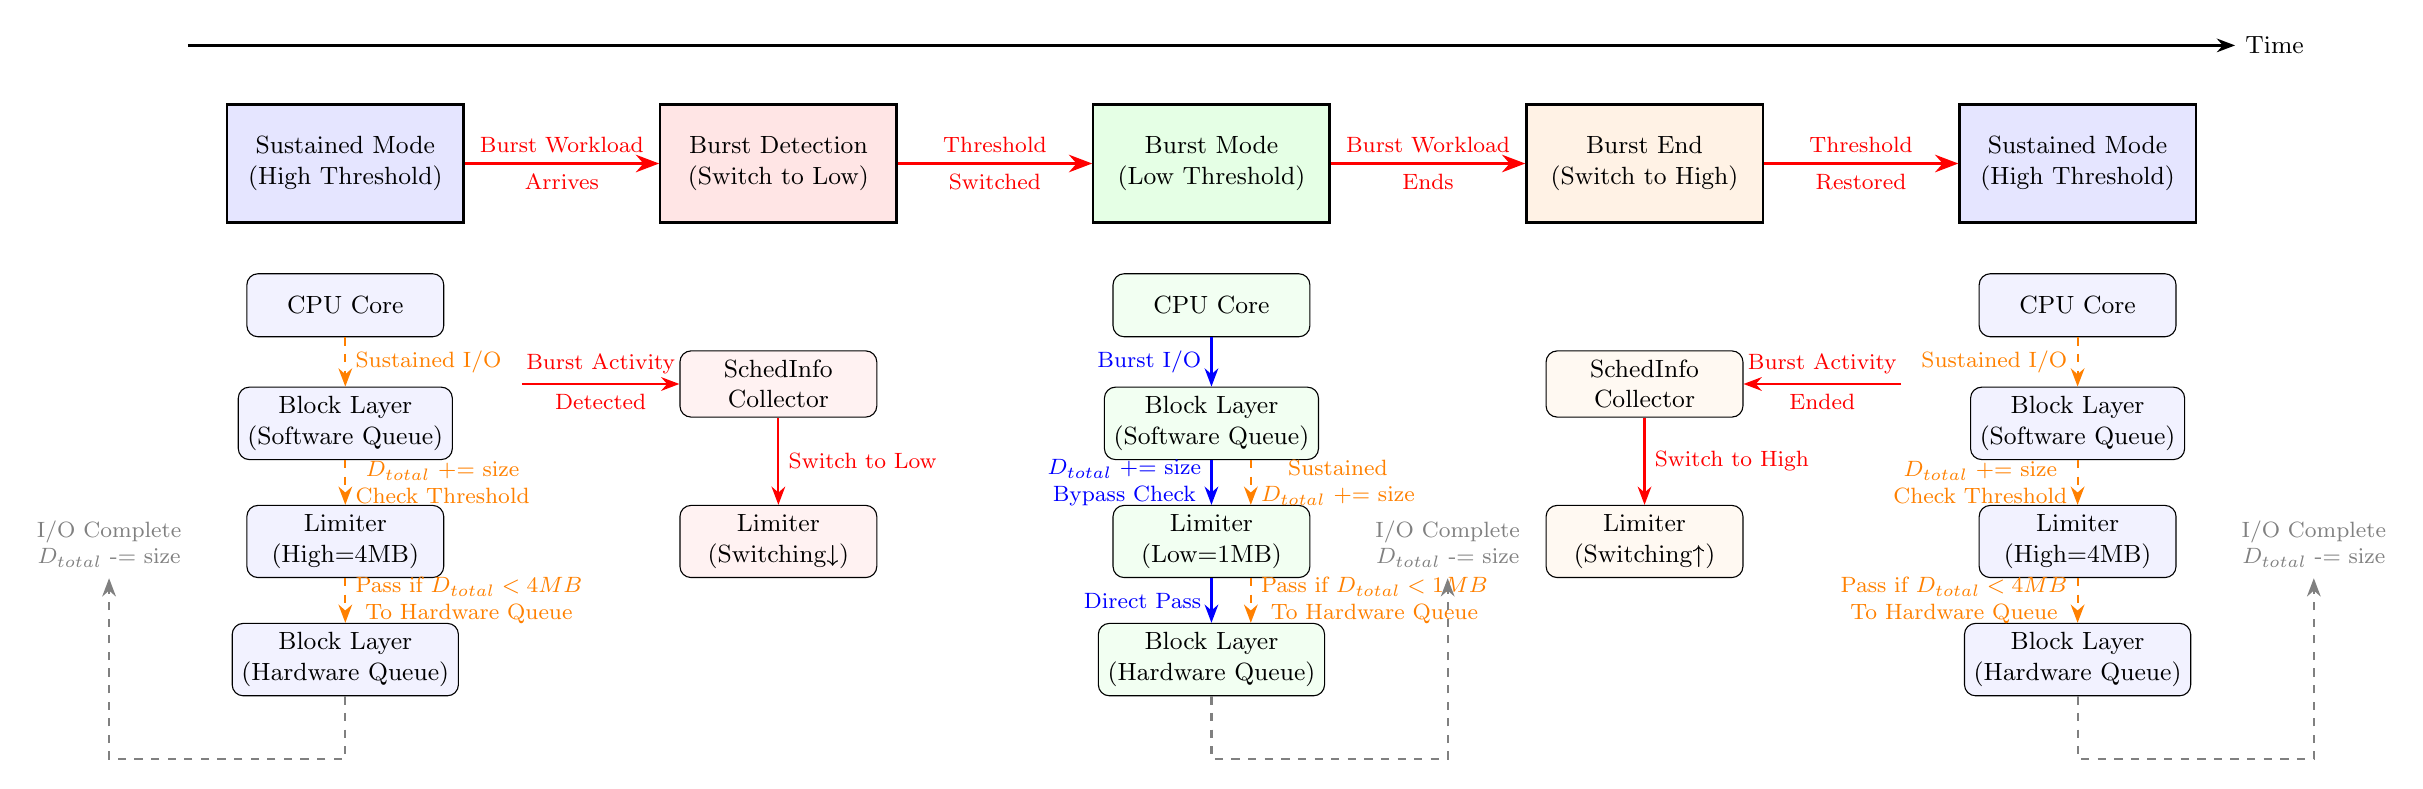
\begin{tikzpicture}[
    font=\small,
    stage/.style={draw, thick, minimum height=1.5cm, minimum width=3cm, align=center},
    io/.style={draw, rounded corners, minimum height=0.8cm, minimum width=2.5cm, align=center},
    burst/.style={-Stealth, thick, blue},
    sustained/.style={-Stealth, thick, dashed, orange},
    inform/.style={-Stealth, thick, red},
    feedback/.style={-Stealth, thick, dashed, gray},
    labelnode/.style={font=\footnotesize, align=center}
]

% Main timeline stages
\node[stage, fill=blue!10] (stage1) at (0,0) {Sustained Mode\\(High Threshold)};
\node[stage, fill=red!10] (stage2) at (5.5,0) {Burst Detection\\(Switch to Low)};
\node[stage, fill=green!10] (stage3) at (11,0) {Burst Mode\\(Low Threshold)};
\node[stage, fill=orange!10] (stage4) at (16.5,0) {Burst End\\(Switch to High)};
\node[stage, fill=blue!10] (stage5) at (22,0) {Sustained Mode\\(High Threshold)};

% First stage I/O flow
\node[io, fill=blue!5] (cpu1) at (0,-1.8) {CPU Core};
\node[io, fill=blue!5] (block1) at (0,-3.3) {Block Layer\\(Software Queue)};
\node[io, fill=blue!5] (limiter1) at (0,-4.8) {Limiter\\(High=4MB)};
\node[io, fill=blue!5] (queue1) at (0,-6.3) {Block Layer\\(Hardware Queue)};

% Second stage (switching to low)
\node[io, fill=red!5] (detector1) at (5.5,-2.8) {SchedInfo\\Collector};
\node[io, fill=red!5] (switch_limiter1) at (5.5,-4.8) {Limiter\\(Switching↓)};

% Third stage I/O flow (burst mode)
\node[io, fill=green!5] (cpu3) at (11,-1.8) {CPU Core};
\node[io, fill=green!5] (block3) at (11,-3.3) {Block Layer\\(Software Queue)};
\node[io, fill=green!5] (limiter3) at (11,-4.8) {Limiter\\(Low=1MB)};
\node[io, fill=green!5] (queue3) at (11,-6.3) {Block Layer\\(Hardware Queue)};

% Fourth stage (switching back to high)
\node[io, fill=orange!5] (detector2) at (16.5,-2.8) {SchedInfo\\Collector};
\node[io, fill=orange!5] (switch_limiter2) at (16.5,-4.8) {Limiter\\(Switching↑)};

% Fifth stage I/O flow (back to normal)
\node[io, fill=blue!5] (cpu5) at (22,-1.8) {CPU Core};
\node[io, fill=blue!5] (block5) at (22,-3.3) {Block Layer\\(Software Queue)};
\node[io, fill=blue!5] (limiter5) at (22,-4.8) {Limiter\\(High=4MB)};
\node[io, fill=blue!5] (queue5) at (22,-6.3) {Block Layer\\(Hardware Queue)};

% I/O flows in stage 1 (normal operation)
\draw[sustained] (cpu1) -- (block1) node[midway, right, labelnode] {Sustained I/O};
\draw[sustained] (block1) -- (limiter1) node[midway, right, labelnode] {$D_{total}$ += size\\Check Threshold};
\draw[sustained] (limiter1) -- (queue1) node[midway, right, labelnode] {Pass if $D_{total} < 4MB$\\To Hardware Queue};

% Burst detection and switching to low
\draw[inform] (detector1) -- (switch_limiter1) node[midway, right, labelnode] {Switch to Low};
\draw[inform] ([xshift=-2cm]detector1.west) -- (detector1.west) node[midway, above, labelnode] {Burst Activity} node[midway, below, labelnode] {Detected};

% I/O flows in stage 3 (burst mode)
\draw[burst] (cpu3) -- (block3) node[midway, left, labelnode] {Burst I/O};
\draw[burst] (block3) -- (limiter3) node[midway, left, labelnode] {$D_{total}$ += size\\Bypass Check};
\draw[sustained] ([xshift=0.5cm]block3.south) -- ([xshift=0.5cm]limiter3.north) node[midway, right, labelnode] {Sustained\\$D_{total}$ += size};
\draw[burst] (limiter3) -- (queue3) node[midway, left, labelnode] {Direct Pass};
\draw[sustained] ([xshift=0.5cm]limiter3.south) -- ([xshift=0.5cm]queue3.north) node[midway, right, labelnode] {Pass if $D_{total} < 1MB$\\To Hardware Queue};

% Burst end detection and switching back to high
\draw[inform] (detector2) -- (switch_limiter2) node[midway, right, labelnode] {Switch to High};
\draw[inform] ([xshift=2cm]detector2.east) -- (detector2.east) node[midway, above, labelnode] {Burst Activity} node[midway, below, labelnode] {Ended};

% I/O flows in stage 5 (back to normal)
\draw[sustained] (cpu5) -- (block5) node[midway, left, labelnode] {Sustained I/O};
\draw[sustained] (block5) -- (limiter5) node[midway, left, labelnode] {$D_{total}$ += size\\Check Threshold};
\draw[sustained] (limiter5) -- (queue5) node[midway, left, labelnode] {Pass if $D_{total} < 4MB$\\To Hardware Queue};

% Timeline arrow
\draw[thick, -Stealth] (-2,1.5) -- (24,1.5) node[right] {Time};

% Stage transitions
\draw[inform, very thick] (stage1.east) -- (stage2.west) node[midway, above, labelnode] {Burst Workload} node[midway, below, labelnode] {Arrives};
\draw[inform, very thick] (stage2.east) -- (stage3.west) node[midway, above, labelnode] {Threshold} node[midway, below, labelnode] {Switched};
\draw[inform, very thick] (stage3.east) -- (stage4.west) node[midway, above, labelnode] {Burst Workload} node[midway, below, labelnode] {Ends};
\draw[inform, very thick] (stage4.east) -- (stage5.west) node[midway, above, labelnode] {Threshold} node[midway, below, labelnode] {Restored};

% Feedback arrows (simplified)
\draw[feedback] (queue1.south) -- ++(0,-0.8) -- ++(-3,0) -- ++(0,2.3) node[above, labelnode] {I/O Complete\\$D_{total}$ -= size};
\draw[feedback] (queue3.south) -- ++(0,-0.8) -- ++(3,0) -- ++(0,2.3) node[above, labelnode] {I/O Complete\\$D_{total}$ -= size};
\draw[feedback] (queue5.south) -- ++(0,-0.8) -- ++(3,0) -- ++(0,2.3) node[above, labelnode] {I/O Complete\\$D_{total}$ -= size};

\end{tikzpicture}
\end{document}